% Options for packages loaded elsewhere
\PassOptionsToPackage{unicode}{hyperref}
\PassOptionsToPackage{hyphens}{url}
%
\documentclass[
]{article}
\usepackage{lmodern}
\usepackage{amsmath}
\usepackage{ifxetex,ifluatex}
\ifnum 0\ifxetex 1\fi\ifluatex 1\fi=0 % if pdftex
  \usepackage[T1]{fontenc}
  \usepackage[utf8]{inputenc}
  \usepackage{textcomp} % provide euro and other symbols
  \usepackage{amssymb}
\else % if luatex or xetex
  \usepackage{unicode-math}
  \defaultfontfeatures{Scale=MatchLowercase}
  \defaultfontfeatures[\rmfamily]{Ligatures=TeX,Scale=1}
\fi
% Use upquote if available, for straight quotes in verbatim environments
\IfFileExists{upquote.sty}{\usepackage{upquote}}{}
\IfFileExists{microtype.sty}{% use microtype if available
  \usepackage[]{microtype}
  \UseMicrotypeSet[protrusion]{basicmath} % disable protrusion for tt fonts
}{}
\makeatletter
\@ifundefined{KOMAClassName}{% if non-KOMA class
  \IfFileExists{parskip.sty}{%
    \usepackage{parskip}
  }{% else
    \setlength{\parindent}{0pt}
    \setlength{\parskip}{6pt plus 2pt minus 1pt}}
}{% if KOMA class
  \KOMAoptions{parskip=half}}
\makeatother
\usepackage{xcolor}
\IfFileExists{xurl.sty}{\usepackage{xurl}}{} % add URL line breaks if available
\IfFileExists{bookmark.sty}{\usepackage{bookmark}}{\usepackage{hyperref}}
\hypersetup{
  pdftitle={Appendix},
  hidelinks,
  pdfcreator={LaTeX via pandoc}}
\urlstyle{same} % disable monospaced font for URLs
\usepackage[margin=1in]{geometry}
\usepackage{graphicx}
\makeatletter
\def\maxwidth{\ifdim\Gin@nat@width>\linewidth\linewidth\else\Gin@nat@width\fi}
\def\maxheight{\ifdim\Gin@nat@height>\textheight\textheight\else\Gin@nat@height\fi}
\makeatother
% Scale images if necessary, so that they will not overflow the page
% margins by default, and it is still possible to overwrite the defaults
% using explicit options in \includegraphics[width, height, ...]{}
\setkeys{Gin}{width=\maxwidth,height=\maxheight,keepaspectratio}
% Set default figure placement to htbp
\makeatletter
\def\fps@figure{htbp}
\makeatother
\setlength{\emergencystretch}{3em} % prevent overfull lines
\providecommand{\tightlist}{%
  \setlength{\itemsep}{0pt}\setlength{\parskip}{0pt}}
\setcounter{secnumdepth}{-\maxdimen} % remove section numbering
\ifluatex
  \usepackage{selnolig}  % disable illegal ligatures
\fi
\newlength{\cslhangindent}
\setlength{\cslhangindent}{1.5em}
\newlength{\csllabelwidth}
\setlength{\csllabelwidth}{3em}
\newenvironment{CSLReferences}[2] % #1 hanging-ident, #2 entry spacing
 {% don't indent paragraphs
  \setlength{\parindent}{0pt}
  % turn on hanging indent if param 1 is 1
  \ifodd #1 \everypar{\setlength{\hangindent}{\cslhangindent}}\ignorespaces\fi
  % set entry spacing
  \ifnum #2 > 0
  \setlength{\parskip}{#2\baselineskip}
  \fi
 }%
 {}
\usepackage{calc}
\newcommand{\CSLBlock}[1]{#1\hfill\break}
\newcommand{\CSLLeftMargin}[1]{\parbox[t]{\csllabelwidth}{#1}}
\newcommand{\CSLRightInline}[1]{\parbox[t]{\linewidth - \csllabelwidth}{#1}\break}
\newcommand{\CSLIndent}[1]{\hspace{\cslhangindent}#1}

\title{Appendix}
\author{}
\date{\vspace{-2.5em}}

\begin{document}
\maketitle

\hypertarget{slice-volume-derivation}{%
\section{Slice volume derivation}\label{slice-volume-derivation}}

The relative volume of a slice through a \(p\) dimensional hypersphere
of radius \(R\) was previously derived in Laa, Cook, and Valencia
(2019). Below we reproduce the calculation for the convenience of the
reader. We start with the volume of the hypersphere with radius \(r\) in
\(q\) dimensions: \begin{equation}
V(r, q) = \frac{\pi^{q/2} r^q}{\frac{q}{2} \Gamma(q/2)}.
\end{equation} The variation of the volume with the radius is given as
\begin{equation}
\frac{dV(r, q)}{dr} = 2 \frac{\pi^{q/2} r^{q-1}}{\Gamma(q/2)}.
\end{equation}

The volume in a slice is spherical in the orthogonal space (\(p-2\)
dimensions) and capturing the full area within the plane. We thus
compute it by integrating the product of \(\frac{dV(r, p-2)}{dr}\) and
the area in the plane parametrised by \(r\). The area in the plane is a
circle with radius \(\sqrt{R^2 - r^2}\). The slice volume is thus
calculated as \begin{equation}
V_{slice}(R, h, p) =
\int_0^h \frac{dV(r, p-2)}{dr} V(\sqrt{R^2 - r^2}, 2) dr =
\frac{\pi^{p/2}}{\Gamma(p/2)} \frac{h^{p-2}}{p} [pR^2 - (p-2)h^2].
\end{equation} The relative volume of the slice given by the fraction
\begin{equation}
V_{rel}(R, h, p) = \frac{V_{slice}(R, h, p)}{V(R, p)} = \frac{h^{p-2}}{2R^p} [pR^2 - (p-2)h^2].
\end{equation}

\hypertarget{simulated-data}{%
\section{Simulated data}\label{simulated-data}}

The four-dimensional hyperspherical harmonics (Domokos 1967) can be
written as \begin{eqnarray}
Z^m_{n\ell}(\beta,\theta,\phi)=2^{\ell+1/2}\sqrt{\frac{(n+1)\Gamma(n-\ell+1)}{\pi\Gamma(n+\ell+2)}}
\Gamma(\ell+1)\sin^\ell\beta C^{(\ell+1)}_{n-\ell}(\cos\beta)Y^m_\ell(\theta,\phi),
\end{eqnarray} where \(C^{(\ell+1)}_{n-\ell}\) are the Gegenbauer
polynomials and \(Y^m_\ell(\theta,\phi)\) are the 3D spherical
harmonics. The polynomials are defined over the 4D unit hypersphere
\(S^3\) in \(\mathbb{R}^4\) and parameterized by three angles: the
azimuthal angles \(\phi\), the 3D zenith (or polar) angle \(\theta\) and
the 4D zenith angle \(\beta\).

The data sets (A, B) are generated from two of these polynomials.
Explicitly they are obtained from, \begin{eqnarray}
{\rm Set~A:}~Z^0_{20} &=& \frac{3-4\sin^2\beta}{\sqrt{2}\pi} \nonumber \\
{\rm Set~B:}~\sqrt{\frac{3}{2}}Z^1_{53} &=& \sqrt{\frac{3}{10}}\frac{1}{2\pi} e^{i\phi}\sin^3\beta\left(40\cos^2\beta-4\right)\sin\theta\left(1-5\cos^2\theta\right)
\end{eqnarray}

To generate the data sets we start from a uniform sample of points
inside a 4-ball of radius one (the inside of the hypersphere \(S^3\))
which we then classify into inside or outside points depending on
whether \(r\) is less than or greater than
\(|Z^m_{n\ell}(\beta,\theta,\phi)|\). This procedure generates a much
larger number of outside than inside points so we collect them
separately to obtain reasonably sized samples. The uniform sampling is
done in Cartesian coordinates \((x,y,z,t)\) which are then transformed
to hyper-spherical coordinates
\((r\cos\beta,r\sin\beta\cos\theta,r\sin\beta\sin\theta\cos\phi,r\sin\beta\sin\theta\sin\phi)\).

\hypertarget{radial-cdf-of-projected-hyperspheres}{%
\section{Radial CDF of projected
hyperspheres}\label{radial-cdf-of-projected-hyperspheres}}

The radial CDF used throughout this work can be derived by calculating
the fraction of the projected volume within a circle of radius \(r\).
The volume of a \(p\) dimensional hypersphere with radius \(R\) is
\begin{equation}
V(p, R) = \frac{2 \pi^{p/2} R^p} {p \Gamma(p/2)}
\end{equation} and the projected volume \textit{outside} a circle of
radius \(r\) is \begin{equation}
V_{outside} (r, p, R) = \int_r^R V(p-2, \sqrt{R^2 - \rho^2}) 2 \pi \rho d\rho =
\frac{\pi^{p/2}(R^4 - r^2 R^2)^{p/2}}{R^p \Gamma(p/2+1)}.
\end{equation} The projected volume \textit{inside} the circle is given
by \begin{equation}
V_{inside}(r, p, R) = V(p, R) - V_{outside}(r, p, R),
\end{equation} and we therefore get the relative volume within the
circle (and thus the radial CDF) as \begin{equation}
F (r, p, R) = \frac{V_{inside}(r, p, R)}{V(p, R)} = 1 - \left(1-\left(\frac{r}{R}\right)^2\right)^{p/2}.
\end{equation}

\hypertarget{squared-masses-in-the-two-higgs-doublet-model}{%
\section{Squared masses in the two-Higgs-doublet
model}\label{squared-masses-in-the-two-higgs-doublet-model}}

Following Gunion and Haber (2003) we compute the squared masses as
\begin{eqnarray}
m_h^2 &=& \frac{v^2}{
     \sin(\beta - \alpha)}~(-\lambda_1\cos^3\beta~
      \sin\alpha + \lambda_2\sin^3\beta\cos\alpha+ 
     \frac{\lambda_{345}}{2}~
      \cos(\beta + \alpha)\sin(2\beta)) \\ \nonumber
m_H^2 &=& \frac{v^2}{
    \cos(\beta - \alpha)}~(\lambda_1\cos^3\beta~
      \cos\alpha + \lambda_2\sin^3\beta\sin\alpha+ 
     \frac{\lambda_{345}}{2}~
      \sin(\beta + \alpha)\sin(2\beta)) \\ \nonumber
m_{H^\pm}^2 &=& \frac{v^2}{ \sin(2(\beta - \alpha))}~(-\sin(
        2\alpha)~(\lambda_1\cos^2\beta - \lambda_2~
         \sin^2\beta) + \lambda_{345}~
      \sin(2\beta)\cos(2\alpha) - \frac{\lambda_{45}}{2}~
       \sin(2(\beta - \alpha))) \\ \nonumber
m_A^2 &=& \frac{v^2}{ \sin(2(\beta - \alpha))}~(\sin(
      2\alpha)~(-\lambda_1\cos^2\beta + \lambda_2~
        \sin^2\beta) + \lambda_{345}~
     \sin(2\beta)\cos(2\alpha) - 
    \lambda_5 \sin(2(\beta - \alpha)))
    \label{masses}
\end{eqnarray}

where we have used the shorthand notation
\(\lambda_{ij\cdots}=\lambda_i+\lambda_j+\cdots\) and the constant
\(v\approx 246\)\textasciitilde GeV sets the scale for the masses.

\hypertarget{additional-application-pdfsense-data}{%
\section{Additional application: PDFSense
data}\label{additional-application-pdfsense-data}}

As similar example, but with different behavior, is given by the
decision boundaries of a classification model for the PDFSense dataset.
This data has 4021 observations in a 56 dimensional parameter space,
that are grouped into 3 classes (Wang et al. 2018). Following the
analysis in Cook, Laa, and Valencia (2018) we only consider the first
six principal components, and train an svm classification model with
radial kernel. We again use classifly and select the resulting sample
points inside a 6D hypersphere after individual centering and scaling
each of the variables.

For this example, the classifier wraps tightly around two of the groups
(DIS and jets), and most of the space is filled by the third group
(VBP). We select only the samples predicting the VBP class, generating a
sample with a small hollow region to be found by section pursuit. We
again use the index with polar binning, with 5 equidistant radial bins
and 8 angular bins. We set \(q=1\) and use the tourr function
search\_better to find the view with the maximum index value.

The result is shown in Fig. \ref{fig:pdffit}, comparing the starting
projection (top row) and the final view (bottom row). In the final slice
view of the classifier predictions we see the decision boundaries
between the three classes. The different regions are hidden in the
projection of the classifier and of the data. In this case the svm model
uses additional information from the orthogonal directions to separate
the three classes. By looking at the final slice from section pursuit we
have obtained a conditional view that allows us to resolve the resulting
boundary.

\begin{figure}
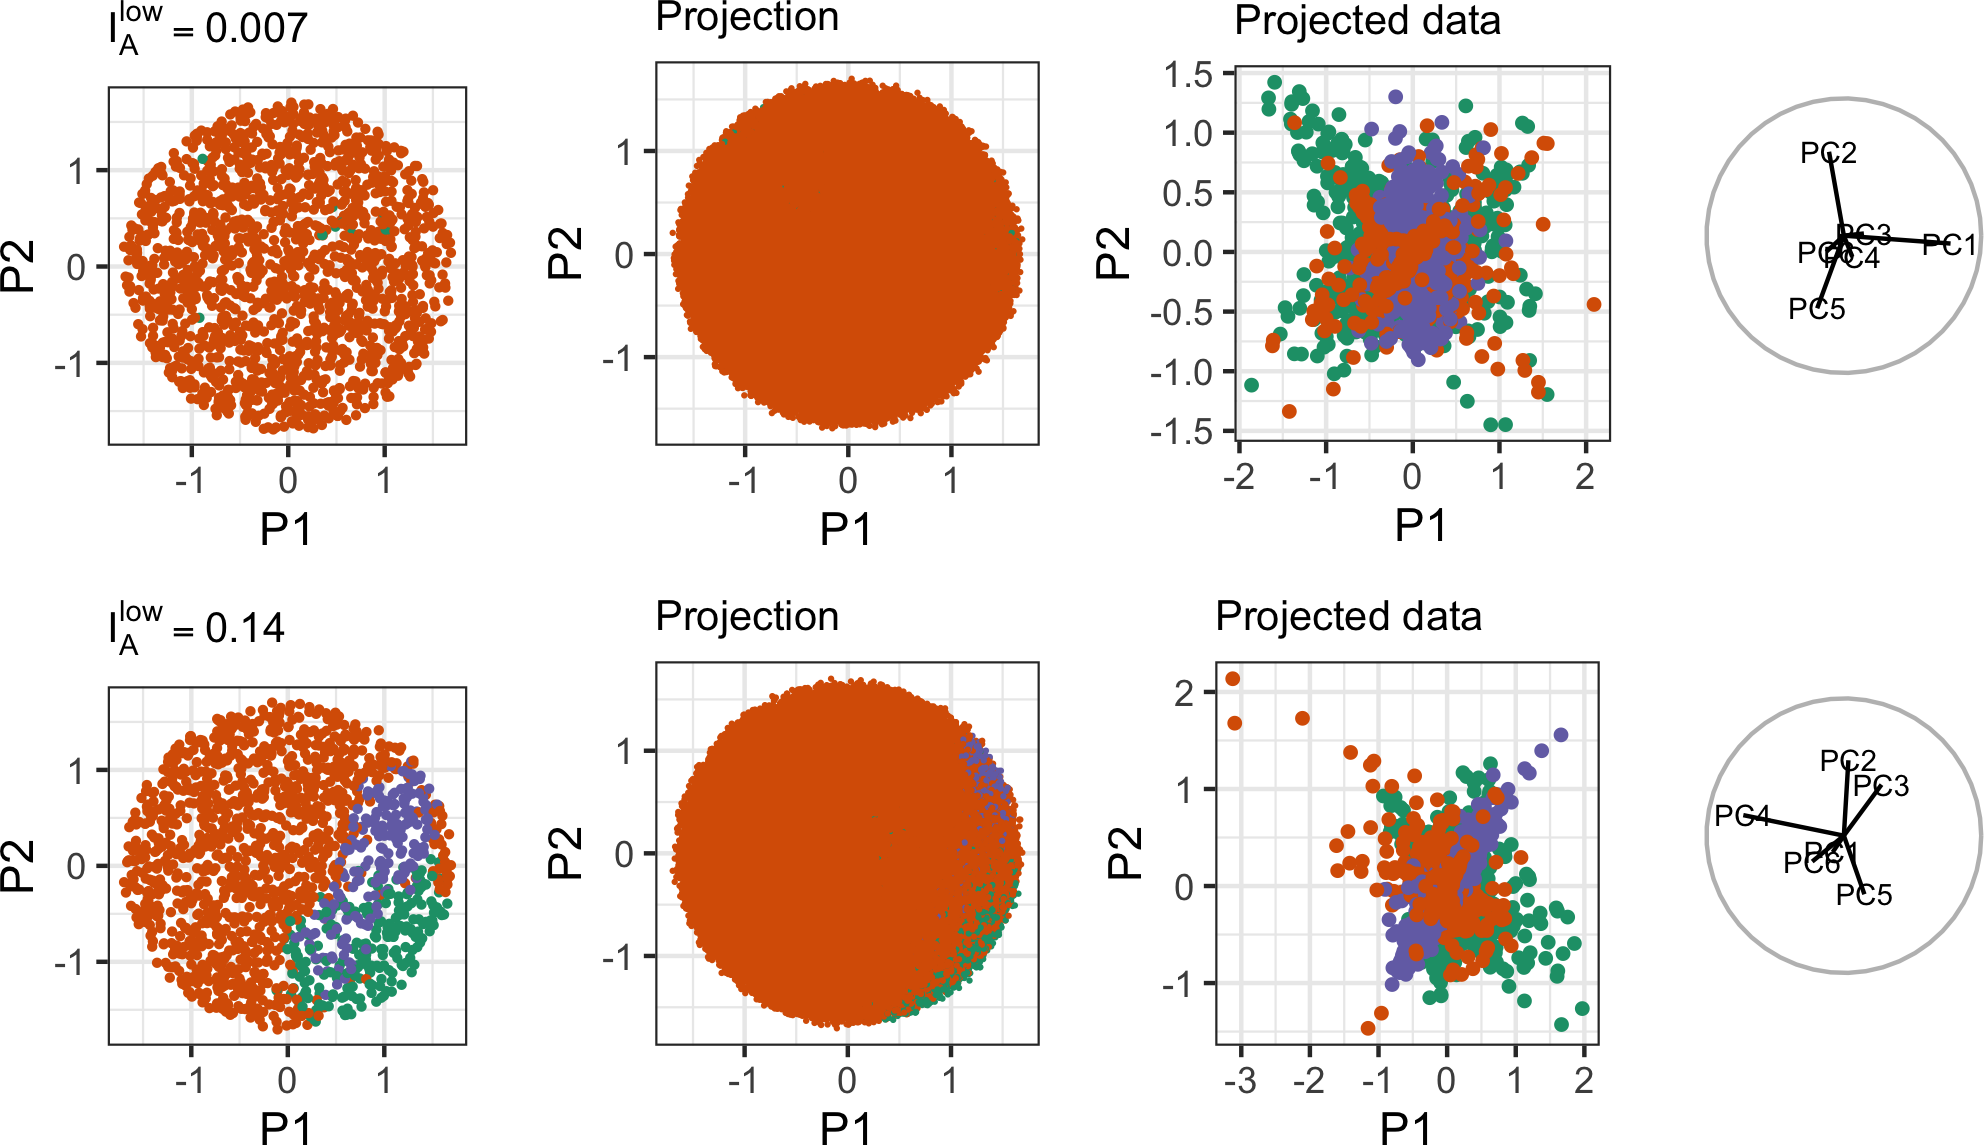
\includegraphics[width=1\linewidth]{appendix_files/figure-latex/pdffit-1} \caption{SVM classification of the PDFSense data, with predicted classes mapped to color. The first row shows a random starting projection, the second row is the final projection obtained via section pursuit on the second class shown in orange. The first and second column show the predicted class label from the svm in a thin slice and a projection. The third column shows the projected data in the same plane, and the last column shows the axes of the corresponding projection.}\label{fig:pdffit}
\end{figure}

\hypertarget{refs}{}
\begin{CSLReferences}{1}{0}
\leavevmode\hypertarget{ref-Cook:2018mvr}{}%
Cook, Dianne, Ursula Laa, and German Valencia. 2018. {``{Dynamical
projections for the visualization of PDFSense data}.''} \emph{Eur. Phys.
J.} C78 (9): 742. \url{https://doi.org/10.1140/epjc/s10052-018-6205-2}.

\leavevmode\hypertarget{ref-Domokos:1967fgx}{}%
Domokos, G. 1967. {``{Four-Dimensional Symmetry}.''} \emph{Phys. Rev.}
159 (5): 1387. \url{https://doi.org/10.1103/PhysRev.159.1387}.

\leavevmode\hypertarget{ref-Gunion:2002zf}{}%
Gunion, John F., and Howard E. Haber. 2003. {``{The CP conserving two
Higgs doublet model: The Approach to the decoupling limit}.''}
\emph{Phys. Rev.} D67: 075019.
\url{https://doi.org/10.1103/PhysRevD.67.075019}.

\leavevmode\hypertarget{ref-laa2019slice}{}%
Laa, Ursula, Dianne Cook, and German Valencia. 2019. {``A Slice Tour for
Finding Hollowness in High-Dimensional Data.''}
\url{https://arxiv.org/abs/1910.10854}.

\leavevmode\hypertarget{ref-Wang:2018heo}{}%
Wang, Bo-Ting, T. J. Hobbs, Sean Doyle, Jun Gao, Tie-Jiun Hou, Pavel M.
Nadolsky, and Fredrick I. Olness. 2018. {``{Mapping the sensitivity of
hadronic experiments to nucleon structure}.''} \emph{Phys. Rev.} D98
(9): 094030. \url{https://doi.org/10.1103/PhysRevD.98.094030}.

\end{CSLReferences}

\end{document}
